\documentclass[11pt,letterpaper]{article}
% PDF reproductible : sans date de compilation ni identifiant aleatoire, pour que git ne voie pas
% de changement quand le contenu est le meme
\pdfinfoomitdate=1
\pdftrailerid{}
\pdfsuppressptexinfo=-1
%graph pour image H
\usepackage{float}

% Pour Dessin
\usepackage{tikz}
\usepackage{amsmath}
\usetikzlibrary{arrows.meta, positioning, patterns}

% packetages pour ecrire en français
\usepackage[french]{babel}
\usepackage[utf8]{inputenc}
\usepackage[T1]{fontenc}

% pour les maths, les graphiques et la navigation dans le pdf
\usepackage{amsmath, amssymb, mathtools, bm, array}
\usepackage{graphicx,caption,subcaption}
\graphicspath{{./}}
\usepackage{pdfpages}
\usepackage{hyperref}
\hypersetup{
    pdftitle={Reconstruction 3D par ultrasons phase array: analyse de la précision spatiale},
    pdfauthor={L-F. Brodeur (LFBRO1), S. L-Tremblay (SILAT10)}
}

% marges, police de caractère et header
\usepackage{geometry}
\geometry{top=23mm, bottom=23mm, left=20mm, right=20mm}
\usepackage{cochineal}
\usepackage{fancyhdr}
\pagestyle{fancy}

\parindent=0mm % pas d'indentation

\lhead{L-F. Brodeur (IDUL: LFBRO1) et S. L-Tremblay (IDUL: SILAT10)}
\rhead{Contrôle non destructif par ultrasons}
\fancyheadoffset{0 cm}

\setlength{\headheight}{13.6pt}

% commandes pour ecrire des equations plus vite avec leur label
\newcommand{\beq}[1]{\begin{equation} \label{#1}}
\def\enq{\end{equation}}

% C'est parti!
\begin{document}
\shorthandoff{;:!?}
\thispagestyle{empty} % pas de header sur la première page
\begin{center}

\noindent
\begin{minipage}[t]{0.5\textwidth}
\raggedright
{\large GPH-3000 \textit{Travaux pratiques avancés}}\\
{\large Automne 2026 $\vert$ GPH-3000 (Groupe: 85213)}
\end{minipage}%
\begin{minipage}[t]{0.5\textwidth}
\raggedleft
{\large \textsc{L-F. Brodeur (IDUL: LFBRO1)}}\\
{\large \textsc{S. L-Tremblay (IDUL: SILAT10)}}
\end{minipage}
\\~\\
\vspace{1em}
{\Large \textbf{Reconstruction 3D par ultrasons phase array:} } \\
{\Large \textbf{analyse de la précision spatiale} } \\[0.3em]
{\large Date du Laboratoire: 24 septembre et 1\textsuperscript{er} octobre 2026 \qquad\qquad Remis le \today}

\end{center}

\vspace{0.5em}
\subsection*{Résumé}
Le son est une onde, et comme toute onde, il interfère avec lui-même. En décalant la phase de plusieurs sources, on peut donc concentrer son énergie en un point choisi, et c'est ce que fait une sonde ultrasonore phase array. Dans cette expérience, un appareil Topaz de Zetec et une sonde linéaire de 64 éléments à 5~MHz ont servi à reconstruire en 3D un bloc d'aluminium avec du texte machiné, en déplaçant la sonde sur sa face plane. Les modèles reconstruits à l'aide de deux méthodes de balayage ont été comparés au modèle CAD de la pièce: une où la position de la sonde est déduite avec l'horloge interne de l'appareil en supposant un déplacement à vitesse constante, et une où la position est directement mesurée par un encodeur à roue. En profondeur, les deux acquisitions mesurent respectivement le dessus de la plaque à $9{,}47 \pm 0{,}20$ et $9{,}60 \pm 0{,}21~\text{mm}$ et le dessus des lettres à $14{,}51 \pm 0{,}30$ et $14{,}76 \pm 0{,}31~\text{mm}$, pour des valeurs CAD de 9,50 et 14,50~mm. Le long du balayage, les mesures dévient plus des valeurs de référence. Sans encodeur, la longueur des lettres varie de 41~\% à 180~\% de leur vraie longueur, à cause de la difficulté d'avancer à exactement 5~mm/s durant le balayage. Avec l'encodeur, les centres des lettres sont placés à 0,3~mm près, mais toutes les distances sont 2,4~\% trop longues, ce qui pointe vers la calibration de l'encodeur. Ce principe de sonde multiéléments vient de la médecine: Somer l'utilisait déjà en 1968 pour faire des échographies du c\oe ur \cite{somer}.

\section{Introduction}

Une sonde ultrasonore conventionnelle ne contient qu'un seul élément piézoélectrique. Elle mesure ce qui se trouve directement sous elle, et il faut la déplacer point par point pour inspecter une surface. Une sonde ultrasonore phase array est plutôt faite d'une rangée d'éléments piézoélectriques. En modifiant la phase entre les éléments, l'appareil peut déplacer le point d'interférence totalement constructive du faisceau, et écouter la réponse après chaque impulsion pour cartographier une coupe complète de la pièce sans bouger la sonde \cite{drinkwater}. Pour obtenir un volume en 3D, il faut quand même déplacer la sonde dans l'autre direction, et connaître sa position à chaque coupe.

L'expérience portait ici sur la qualité de ce volume 3D reconstruit. La sonde a été déplacée à la main sur un bloc d'aluminium usiné dont un modèle CAD donne toutes les dimensions. La question était de savoir avec quelle précision le volume reconstruit reproduit la pièce, en profondeur, le long de la sonde et le long du balayage, et si l'ajout d'un encodeur de position améliore cette précision.

Le principe des sondes multiéléments et des deux façons de positionner la sonde est présenté à la Section~\ref{sec:theorie}. La Section~\ref{sec:methodologie} décrit la pièce, les acquisitions et l'analyse. Les résultats sont présentés à la Section~\ref{sec:resultats}. Ils sont discutés à la Section~\ref{sec:discussion}. La Section~\ref{sec:conclusion} conclut.

\section{Théorie}
\label{sec:theorie}

\subsection{Sonde multiéléments et balayage linéaire}

Chaque élément de la sonde peut être excité avec un délai qui lui est propre. Pour focaliser le faisceau en un point situé à une profondeur $F$, l'élément le plus loin du point focal est excité en premier, et chaque autre élément est retardé de
\beq{eq:loi}
    \tau_i = \frac{r_{\max} - r_i}{c} ,
\enq
où $r_i$ est la distance entre l'élément $i$ et le point focal, $r_{\max}$ la plus grande de ces distances et $c$ la vitesse du son \cite{olympus}. Les ondes de tous les éléments arrivent donc en phase au point focal. L'ensemble des délais forme ce qu'on appelle une loi focale.

En balayage linéaire, un groupe d'éléments voisins (l'ouverture) tire avec la même loi focale, puis le groupe se décale d'un élément le long de la sonde et tire à nouveau. Chaque position du groupe donne un faisceau, et donc les faisceaux sont espacés d'un pas $p$. Le long de la sonde, la largeur du faisceau au point focal est d'environ \cite{olympus}
\beq{eq:largeur}
    \delta \approx \frac{\lambda F}{D} ,
\enq
où $\lambda$ est la longueur d'onde et $D$ la largeur de l'ouverture. Dans l'autre direction, le faisceau n'est pas focalisé: sa largeur est fixée par la largeur des éléments, qui est de 10~mm pour la sonde utilisée. On s'attend donc à une image plus floue le long du balayage que le long des éléments de la sonde.

\subsection{Profondeur d'un écho}

La sonde est fixée sur un sabot droit en plastique, qui envoie une onde sonore à incidence normale dans la pièce. Un écho qui revient après un temps $t$ vient d'une profondeur
\beq{eq:profondeur}
    d = \frac{v\,t}{2} ,
\enq
où $v$ est la vitesse du son dans la pièce (6320~m/s pour une onde sonore dans l'aluminium \cite{krautkramer}). La calibration du Topaz fixe $v$ avec deux échos de fond d'un bloc d'épaisseur connue, et le zéro de profondeur avec une calibration qui sert à caractériser le délai provenant du sabot \cite{protocole_topaz}.

\subsection{Position le long du balayage: horloge vs. encodeur}
\label{sec:theorie_position}

Dans les deux méthodes utilisées ici, la sonde est déplacée à la main. Sans encodeur, le Topaz enregistre une nouvelle position à chaque coup de son horloge interne, à la fréquence d'acquisition $f$. Cette méthode suppose donc que deux coups successifs sont séparés d'un pas $\Delta s$ fixe, c'est-à-dire que la sonde est déplacée à la vitesse $v_{\text{main}} = \Delta s\, f$. Les variations de cette vitesse le long du balayage agissent comme un facteur multiplicatif sur les longueurs mesurées le long du balayage.

Avec un encodeur, une roue fixée au sabot compte des pas lorsque la sonde avance. Dans cette méthode, la position est obtenue en divisant ce compte par la résolution de l'encodeur, obtenue lors d'une calibration sur une distance connue. Le Topaz assigne donc chaque tranche du balayage à une position, avec un pas $\Delta s$. Si la sonde parcourt un pas $\Delta s$ en moins de temps qu'une période d'acquisition ($1/f$, où $f$ est la fréquence d'acquisition maximale), certaines positions ne reçoivent aucune tranche et restent vides. La vitesse de déplacement maximale sans trou est
\beq{eq:vmax}
    v_{\max} = \Delta s\, f .
\enq

\section{Méthodologie}
\label{sec:methodologie}

\subsubsection*{Pièce}
La pièce est une plaque d'aluminium usinée de $140 \times 24 \times 9{,}5~\text{mm}$, sur laquelle sept lettres sont machinées en relief sur 5~mm (Figure~\ref{fig:bloc}). Les lettres ont une hauteur de 18~mm et une longueur de 11,2 à 14,2~mm. La sonde est posée sur la face plane, avec du gel couplant. Là où il n'y a pas de lettre, le son revient sur le dessus de la plaque, à 9,5~mm. Sous une lettre, le son continue dans la lettre et revient sur son dessus, à 14,5~mm.

\begin{figure}[htbp]
    \centering
    \begin{subfigure}[b]{\textwidth}
        \centering
        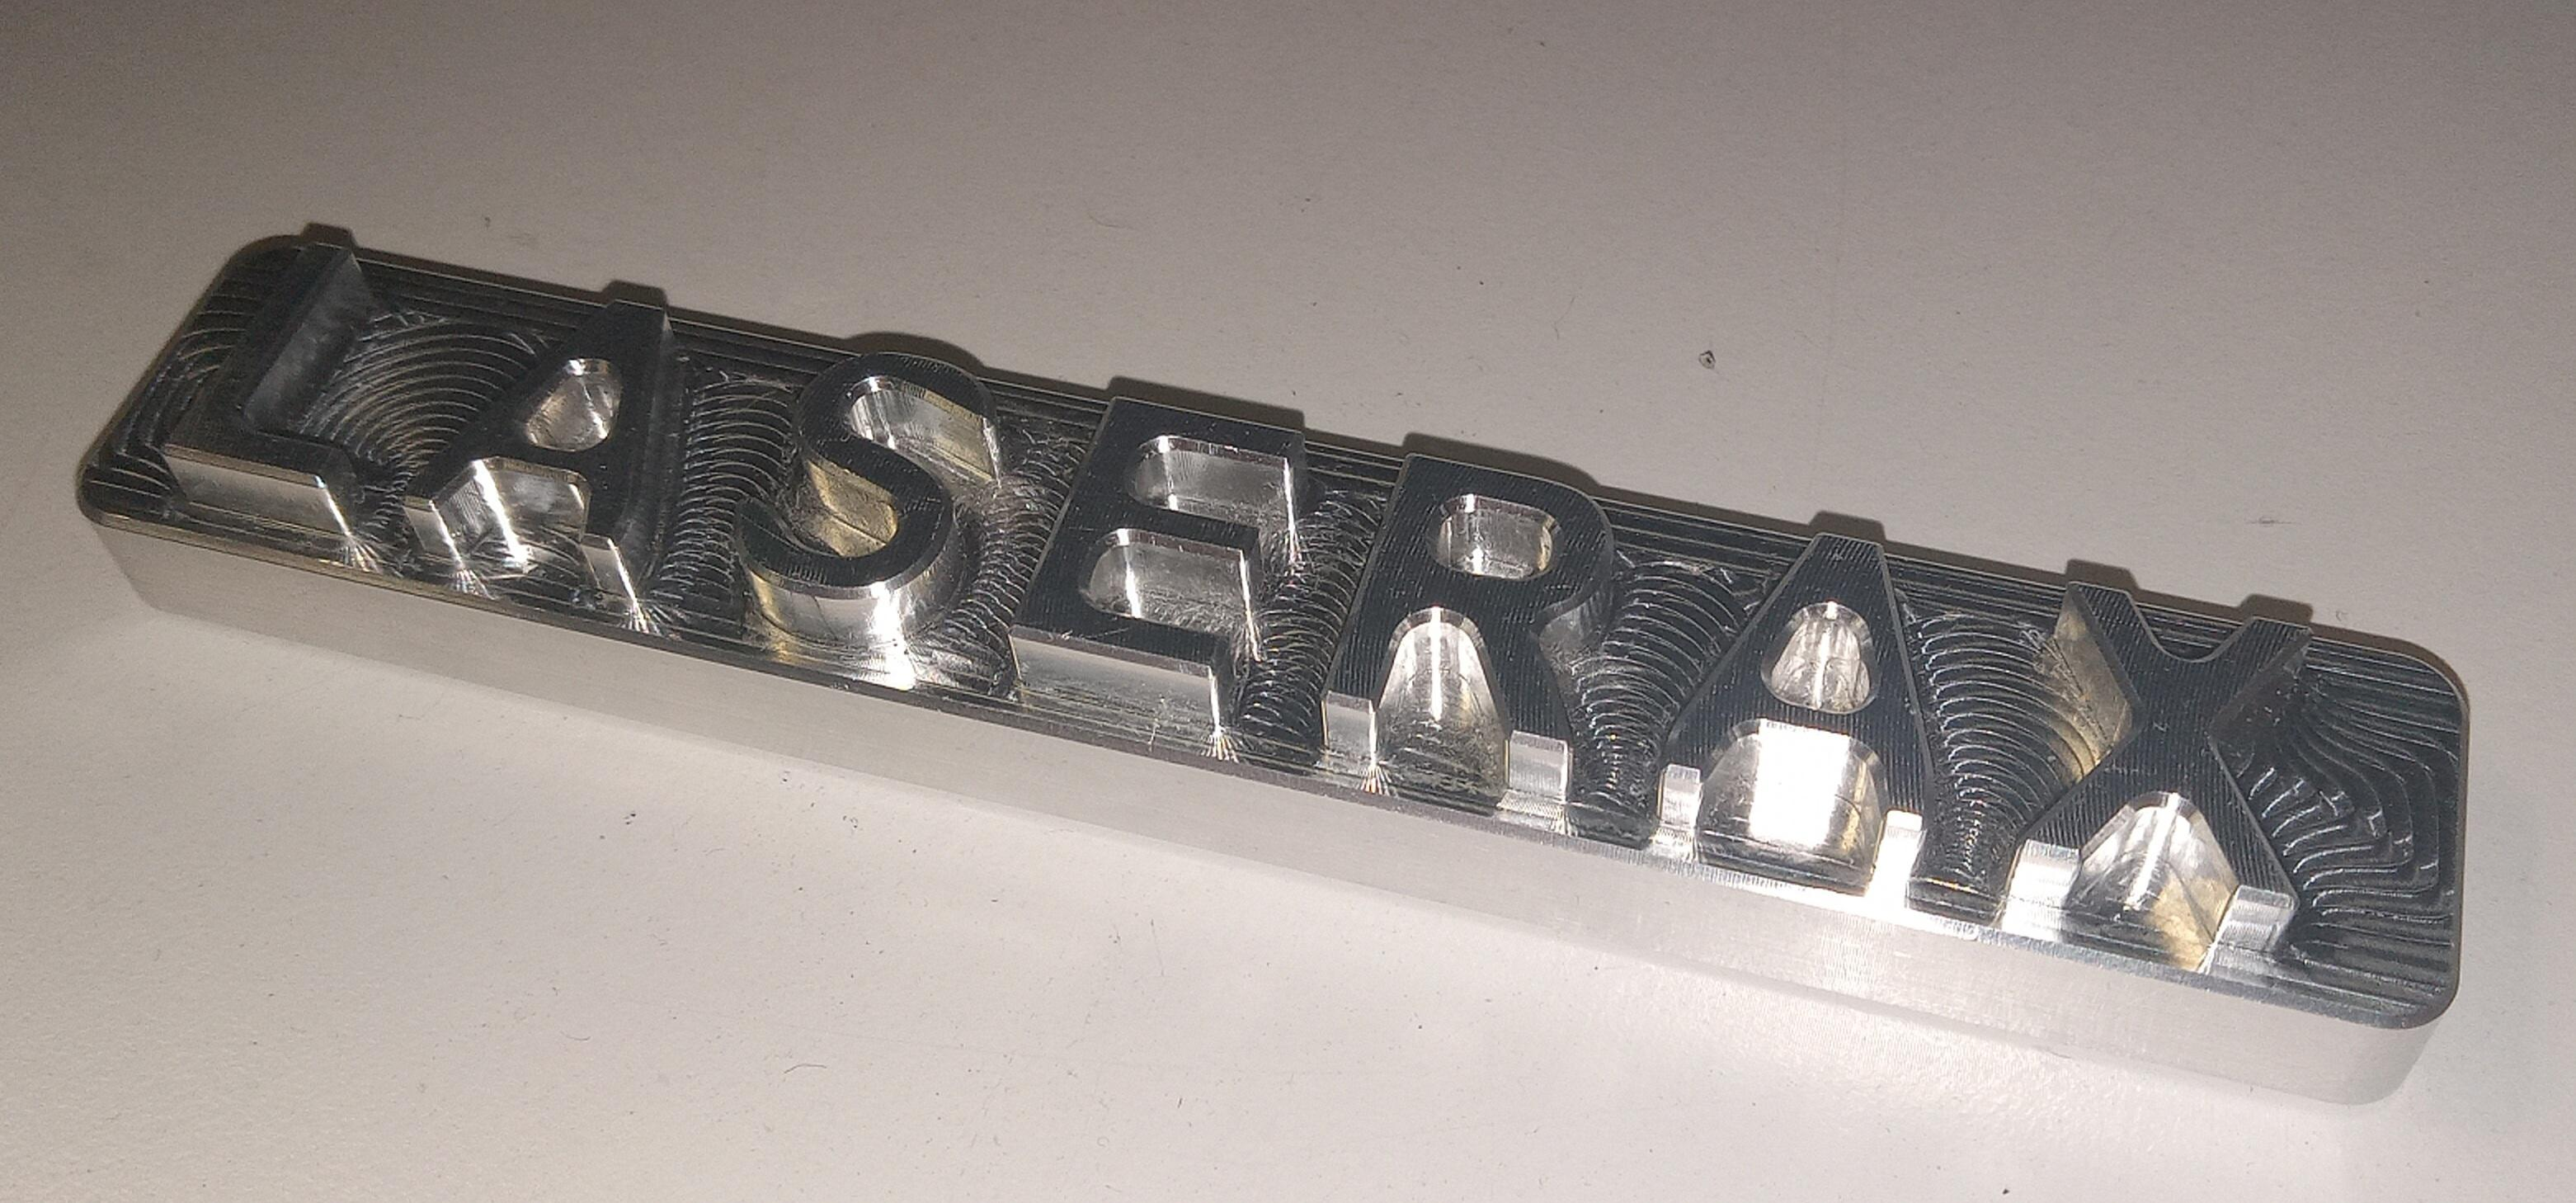
\includegraphics[width=0.62\textwidth]{../figures/Photos_Lab/BlocMachine.jpg}
        \caption{}
        \label{fig:bloc}
    \end{subfigure}
    \\[0.6em]
    \begin{subfigure}[b]{0.5\textwidth}
        \centering
        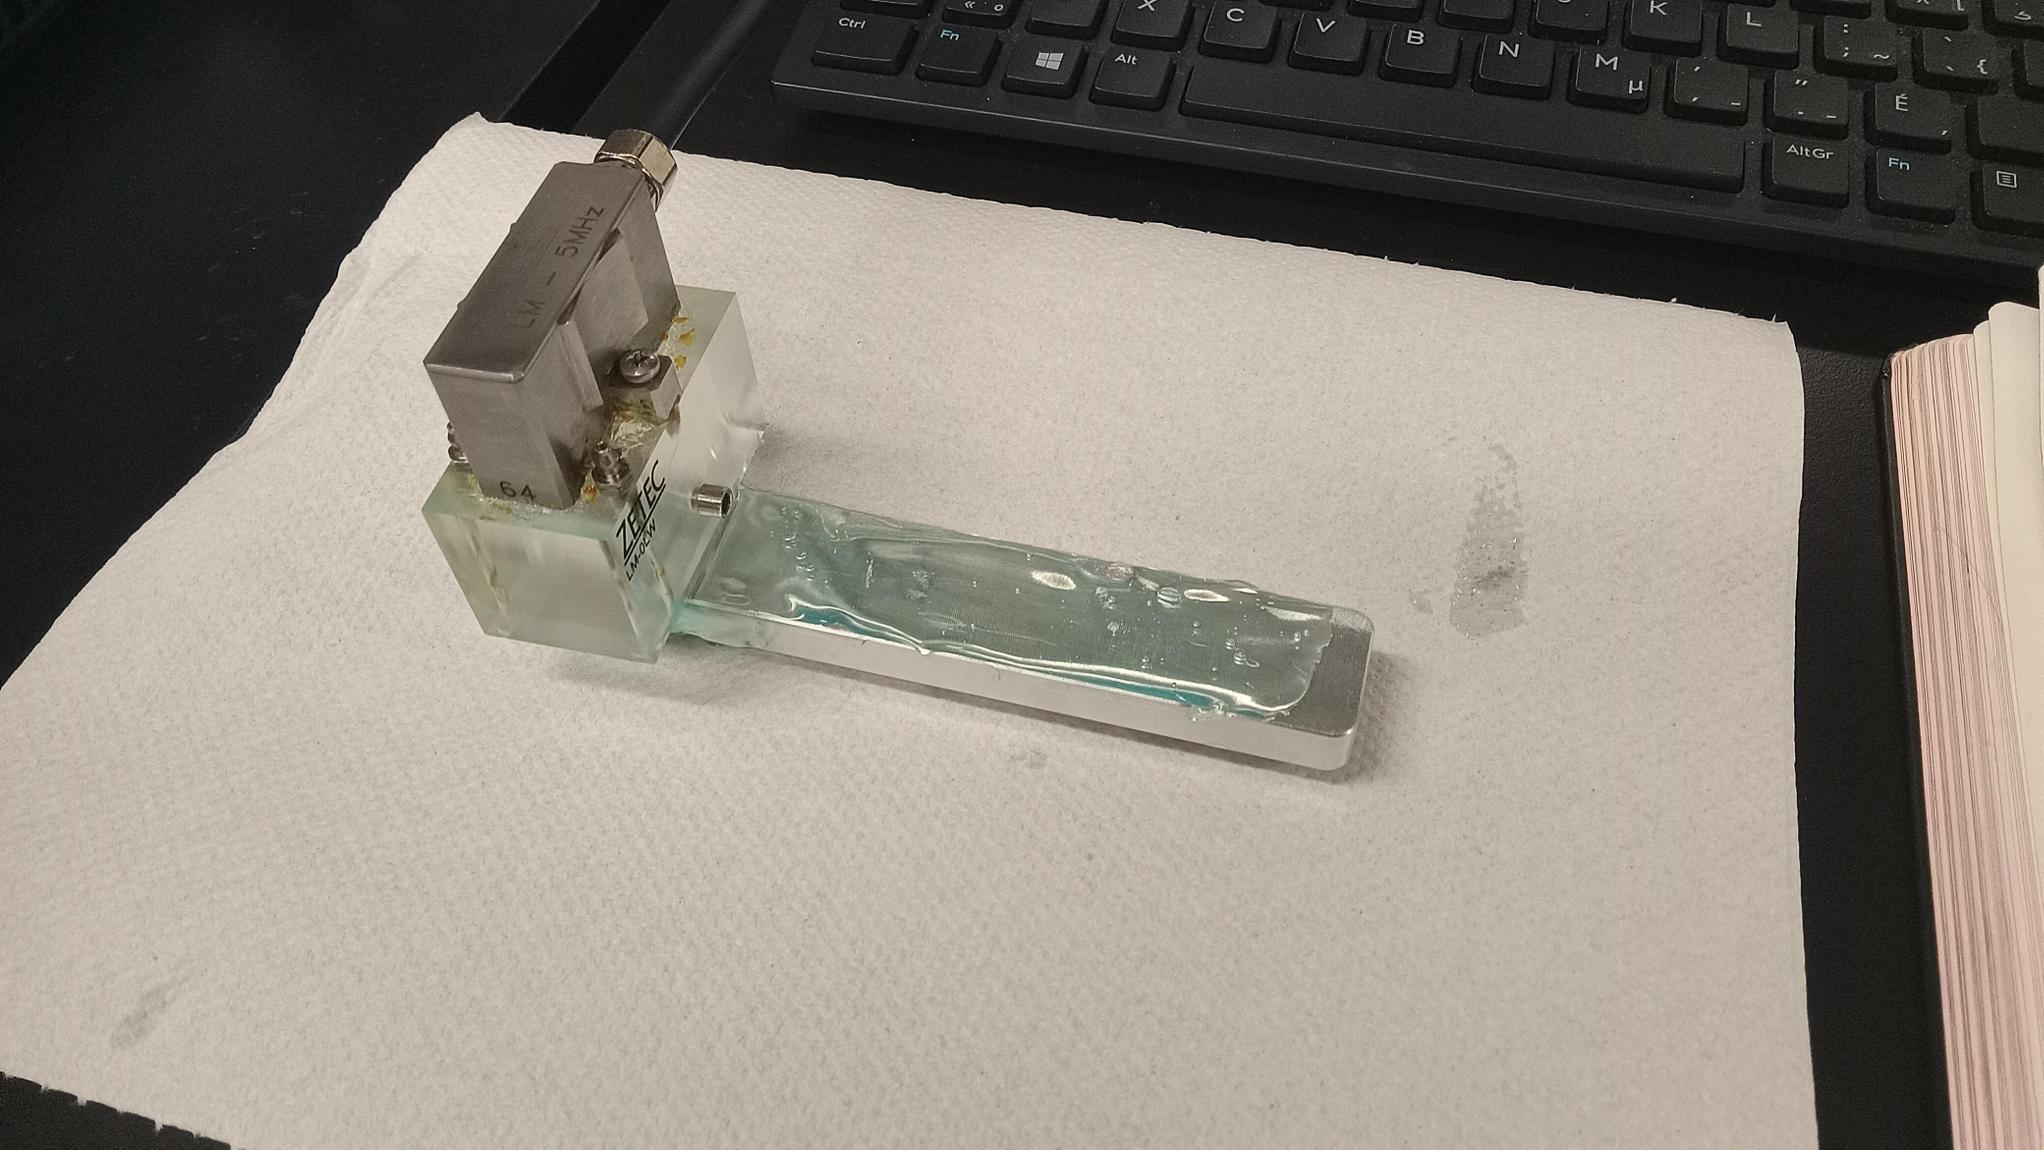
\includegraphics[height=4.2cm]{../figures/Photos_Lab/Methode3.jpg}
        \caption{}
        \label{fig:photo}
    \end{subfigure}
    \hfill
    \begin{subfigure}[b]{0.46\textwidth}
        \centering
        \begin{tikzpicture}[x=0.12cm, y=0.155cm]
            % sabot et sonde
            \fill[cyan!12] (2,0) rectangle (30,6);
            \draw (2,0) rectangle (30,6);
            \fill[gray!45] (9,6) rectangle (23,9.5);
            \draw (9,6) rectangle (23,9.5);
            \node[font=\scriptsize] at (16,7.75) {sonde};
            \node[font=\scriptsize] at (16,3) {sabot};
            % plaque et lettre
            \fill[gray!20] (-4,0) rectangle (36,-9.5);
            \fill[gray!20] (17,-9.5) rectangle (29,-14.5);
            \draw (-4,0) -- (36,0) -- (36,-9.5) -- (29,-9.5) -- (29,-14.5) -- (17,-14.5) -- (17,-9.5) -- (-4,-9.5) -- cycle;
            % trajets
            \draw[-{Latex[length=1.5mm]}, blue!70!black, thick] (8,0) -- (8,-9.3);
            \draw[-{Latex[length=1.5mm]}, blue!70!black, thick] (9.5,-9.3) -- (9.5,0);
            \draw[-{Latex[length=1.5mm]}, orange!85!black, thick] (21.5,0) -- (21.5,-14.3);
            \draw[-{Latex[length=1.5mm]}, orange!85!black, thick] (23,-14.3) -- (23,0);
            % cotes
            \draw[|-|, thin] (-7,0) -- (-7,-9.5) node[midway, left, font=\scriptsize] {9,5 mm};
            \draw[|-|, thin] (39,0) -- (39,-14.5) node[midway, right, font=\scriptsize] {14,5 mm};
            \node[font=\scriptsize, align=center] at (23,-17) {lettre};
            \node[font=\scriptsize] at (6,-12) {plaque};
            \draw[-{Latex[length=1.5mm]}] (-4,-19) -- (8,-19) node[right, font=\scriptsize] {$x$, balayage};
        \end{tikzpicture}
        \caption{}
        \label{fig:schema}
    \end{subfigure}
    \caption{Bloc usiné (a). Sonde et sabot sur la face plane du bloc, avec le gel couplant (b). Coupe du bloc le long du balayage (c).}
    \label{fig:montage}
\end{figure}

\subsubsection*{Acquisitions}
Les mesures ont été faites avec un Topaz16 et le logiciel UltraVision Touch 3.8R11, une sonde linéaire LM de 5~MHz à 64 éléments et le sabot LM-0LW, selon le protocole de l'Annexe~\ref{ann:protocole} \cite{protocole_topaz}. Les trois calibrations (vitesse, délai du sabot, sensibilité) ont été faites sur un bloc d'aluminium de 25,16~mm, et la calibration de vitesse a donné $v = 6451~\text{m/s}$. Plusieurs balayages de pratique ont été faits avec et sans encodeur, et le meilleur de chaque type est analysé ici (Tableau~\ref{tab:acquisitions}). Sans encodeur, des repères de ruban adhésif placés tous les 10~mm aidaient à garder la vitesse visée de 5~mm/s. Pour l'acquisition avec encodeur, le montage incluait aussi le bout d'un autre bloc, qui servait de rail pour guider la sonde le long du balayage et limiter son déplacement en largeur.

\begin{table}[htbp]
\centering
\caption{Paramètres des deux acquisitions analysées (horloge et encodeur).}
\label{tab:acquisitions}
\small
\begin{tabular}{lcc}
\hline
 & Horloge & Encodeur \\
\hline
Source de la position & horloge interne & encodeur à roue (18,68 pas/mm) \\
Fréquence d'acquisition & 20~Hz & 51~Hz \\
Pas de balayage $\Delta s$ & 0,25~mm (supposé) & 0,25~mm \\
Positions enregistrées & 462 & 578, dont 29 vides \\
\hline
\end{tabular}
\end{table}

\subsubsection*{Analyse}
Les données brutes ont été lues et analysées en Python. Les positions vides de l'encodeur sont comblées par interpolation entre les positions voisines. Dans chaque A-scan, on cherche l'écho du dessus de la plaque entre 7,5 et 12~mm, et celui du dessus des lettres entre 12,5 et 17~mm. La profondeur d'un écho est le centre de la partie de l'écho qui dépasse la moitié de son maximum.

Pour l'image dans le plan, on utilise la chute de l'écho de fond, $q = 1 - A/A_{\text{ref}}$, où $A$ est l'amplitude de l'écho du dessus de la plaque et $A_{\text{ref}}$ sa valeur sur la plaque pour le même faisceau. On a $q = 0$ sur la plaque et $q = 1$ sous une lettre. Le seuil $q = 0{,}5$ correspond à la méthode de la chute de 6~dB utilisée en contrôle par ultrasons pour trouver le bord d'un réflecteur \cite{krautkramer}. La carte de $q$ peut ensuite être comparée au CAD. Pour mesurer chaque lettre, sa position et sa distorsion dans les deux axes sont ajustées manuellement, et l'étirement obtenu donne sa longueur et sa hauteur mesurées.

\subsubsection*{Incertitudes}
L'incertitude sur une profondeur (éq.~\ref{eq:profondeur}) vient de la vitesse du son et du temps d'arrivée:
\beq{eq:dd}
    \Delta d = \sqrt{\left(\frac{\partial d}{\partial v}\Delta v\right)^2 + \left(\frac{\partial d}{\partial t}\Delta t\right)^2} = \frac{1}{2}\sqrt{\left(t\,\Delta v\right)^2 + \left(v\,\Delta t\right)^2} .
\enq
On prend $\Delta v = 131~\text{m/s}$, l'écart entre la vitesse calibrée et la vitesse nominale de l'aluminium, et $\Delta t = 20~\text{ns}$, la moitié de la période d'échantillonnage. Une longueur ou une hauteur de lettre est la différence entre les positions de ses deux bords, chacune connue à un pas d'échantillonnage $\Delta x$ près, donc $\Delta L = \sqrt{2}\,\Delta x$, soit 0,35~mm le long du balayage ($\Delta x = 0{,}25~\text{mm}$) et 0,85~mm le long de la sonde ($\Delta x = 0{,}6~\text{mm}$).

\section{Résultats}
\label{sec:resultats}

\subsection{Profondeur}
\label{sec:res_profondeur}

La Figure~\ref{fig:ascans} montre les A-scans moyens sur la plaque et sous les lettres. Sur la plaque, l'écho de fond sort près de 9,5~mm, suivi de son deuxième écho près de 19~mm. Sous une lettre, un écho plus faible sort près de 14,5~mm. Les profondeurs mesurées sont données au Tableau~\ref{tab:profondeur}. Toutes les valeurs correspondent au CAD à l'intérieur de leur incertitude. L'écart entre les deux échos de fond est le même dans les deux acquisitions (9,68~mm).

\begin{figure}[htbp]
    \centering
    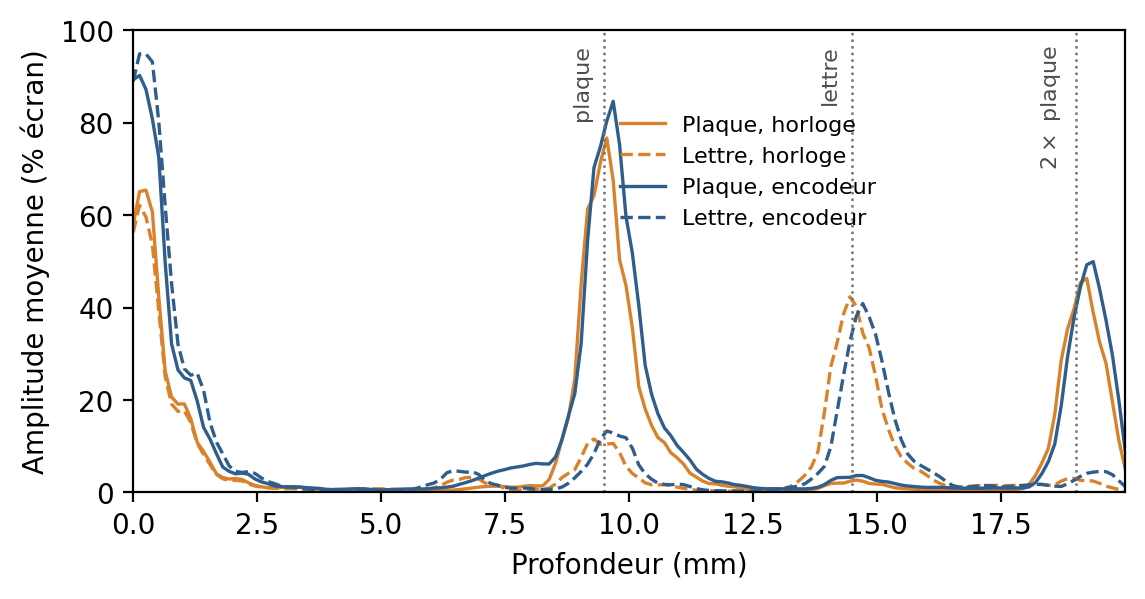
\includegraphics[width=0.66\textwidth]{../figures/02_ascans_profondeur.png}
    \caption{A-scans moyens sur la plaque (traits pleins) et sous les lettres (tirets), sans encodeur (orange) et avec encodeur (bleu).}
    \label{fig:ascans}
\end{figure}

\begin{table}[htbp]
\centering
\caption{Profondeurs mesurées comparées au CAD. Les incertitudes viennent de l'équation~\ref{eq:dd}.}
\label{tab:profondeur}
\small
\begin{tabular}{lccc}
\hline
Grandeur (mm) & CAD & Horloge & Encodeur \\
\hline
Dessus de la plaque & 9,50 & $9{,}47 \pm 0{,}20$ & $9{,}60 \pm 0{,}21$ \\
Dessus des lettres & 14,50 & $14{,}51 \pm 0{,}30$ & $14{,}76 \pm 0{,}31$ \\
Hauteur des lettres (différence) & 5,00 & $5{,}03 \pm 0{,}14$ & $5{,}17 \pm 0{,}14$ \\
Écart entre le 1\textsuperscript{er} et le 2\textsuperscript{e} écho de fond & 9,50 & $9{,}68 \pm 0{,}22$ & $9{,}68 \pm 0{,}22$ \\
\hline
\end{tabular}
\end{table}

\subsection{Forme des lettres dans le plan}

La Figure~\ref{fig:cscans} compare la chute de l'écho de fond au CAD, et la Figure~\ref{fig:3d} montre les surfaces 3D reconstruites sous la surface du CAD. Avec l'encodeur, les sept lettres se lisent et leur forme ne comporte aucune distorsion majeure. Sans encodeur, les lettres sont étirées ou écrasées selon l'endroit, et la fin du mot arrive vers $x = 40~\text{mm}$ au lieu de $60~\text{mm}$ parce que le balayage paraît plus court qu'il ne l'est. Le L, au tout début du balayage, paraît presque deux fois trop long, parce que la sonde, déplacée à la main, avançait trop lentement au départ.

\begin{figure}[htbp]
    \centering
    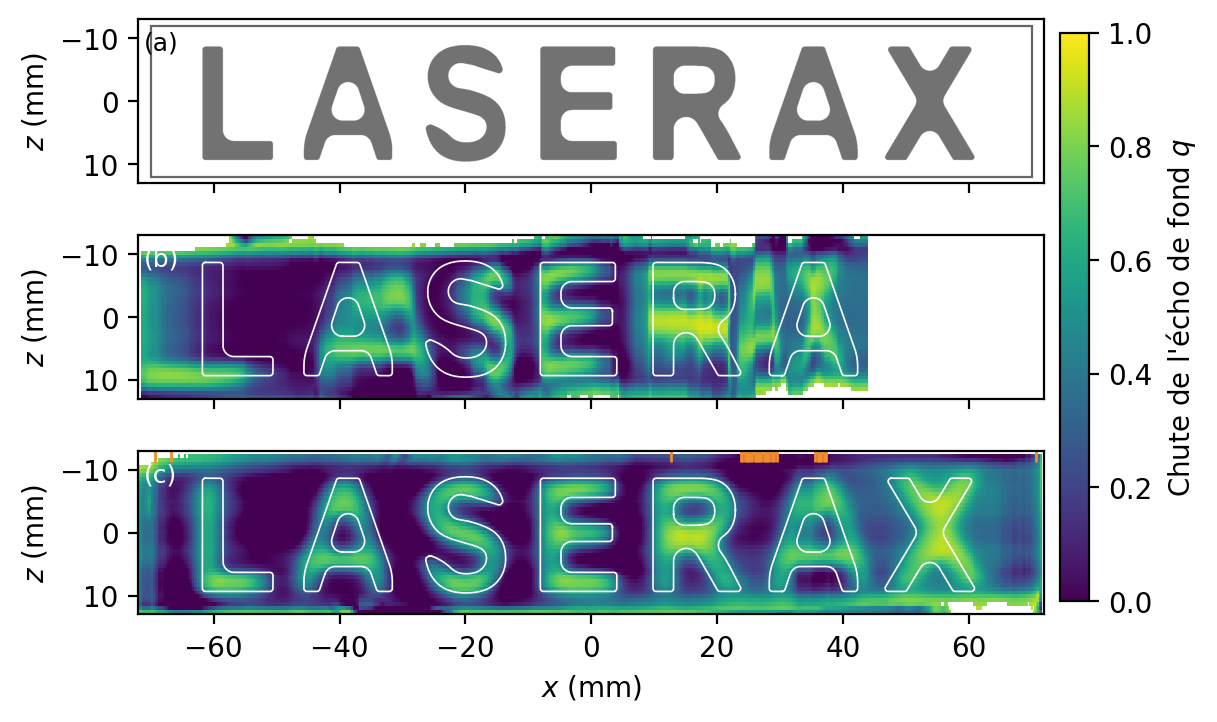
\includegraphics[width=0.84\textwidth]{../figures/01_cscans_cad.png}
    \caption{Lettres du CAD (a) et chute de l'écho de fond $q$ sans encodeur (b) et avec encodeur (c).}
    \label{fig:cscans}
\end{figure}

\begin{figure}[htbp]
    \centering
    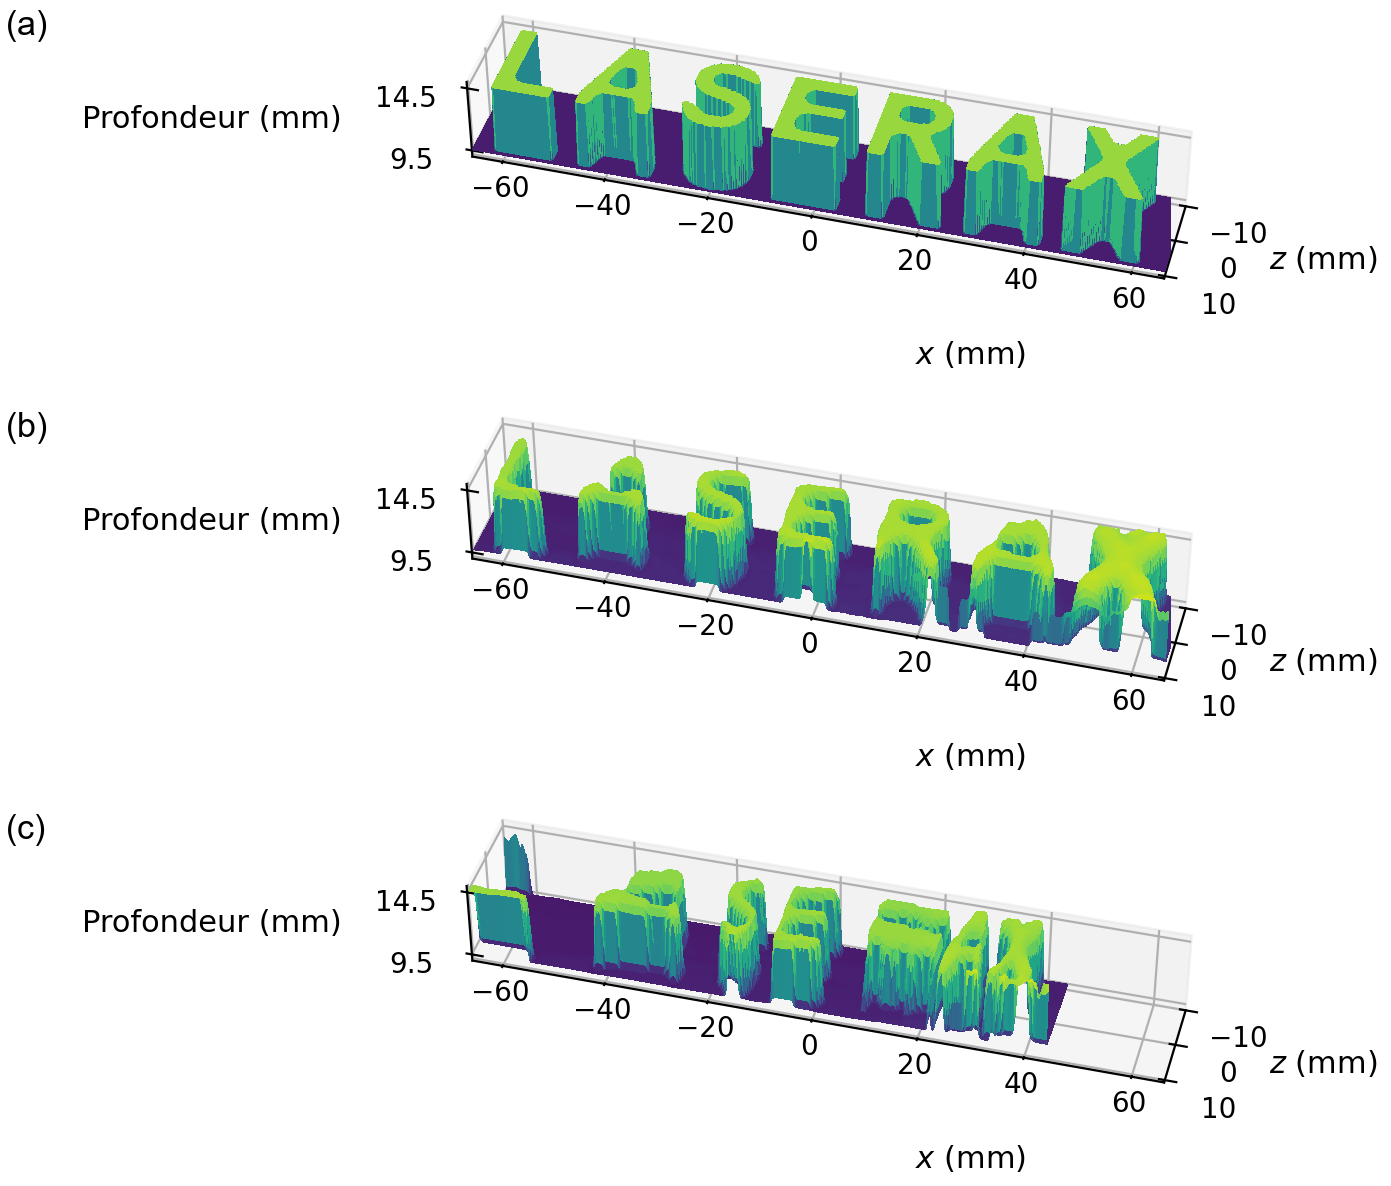
\includegraphics[width=0.66\textwidth]{../figures/04_surfaces_3d_cad_encodeur_horloge.png}
    \caption{Surface du CAD (a) et surfaces reconstruites avec encodeur (b) et sans encodeur (c).}
    \label{fig:3d}
\end{figure}

\subsection{Longueurs, hauteurs et distorsion}
\label{sec:res_plan}

Le Tableau~\ref{tab:lettres} donne la longueur (le long du balayage) et la hauteur (le long de la sonde) de chaque lettre. Le long de la sonde, les deux acquisitions donnent des hauteurs proches de 18~mm, à environ 1~mm près pour la plupart des lettres. Le long du balayage, les longueurs avec encodeur sont un peu plus courtes que le CAD, de 0,2 à 0,8~mm, sauf pour le deuxième A qui est 2,3~mm trop long. Sans encodeur, les longueurs vont de 41~\% (X) à 180~\% (L) de la longueur CAD (Figure~\ref{fig:positions}). En divisant la vitesse supposée de 5~mm/s par cet étirement, on obtient la vitesse de la main sur chaque lettre: elle a varié entre 2,8~mm/s (L) et 12,1~mm/s (X), sur un balayage de 23~s. Le R n'est pas mesuré sans encodeur, parce que la vitesse de la main a changé pendant son passage: il est étiré d'un côté et écrasé de l'autre, et aucun étirement unique ne donne son contour assez précisément.

\begin{table}[htbp]
\centering
\caption{Longueur et hauteur de chaque lettre (mm). L'incertitude est de 0,35~mm sur les longueurs et de 0,85~mm sur les hauteurs.}
\label{tab:lettres}
\small
\begin{tabular}{lcccccc}
\hline
 & \multicolumn{3}{c}{Longueur (le long du balayage)} & \multicolumn{3}{c}{Hauteur (le long de la sonde)} \\
Lettre & CAD & Horloge & Encodeur & CAD & Horloge & Encodeur \\
\hline
L & 11,2 & 20,2 & 10,8 & 18,0 & 18,0 & 20,4 \\
A & 14,1 & 19,8 & 13,9 & 18,0 & 16,9 & 18,0 \\
S & 12,7 & 7,2  & 11,9 & 18,5 & 18,1 & 18,8 \\
E & 12,2 & 11,9 & 11,4 & 18,0 & 18,5 & 18,5 \\
R & 14,0 & n.m.\textsuperscript{a} & 13,2 & 18,0 & n.m.\textsuperscript{a} & 18,7 \\
A & 14,1 & 6,8  & 16,3 & 18,0 & 17,8 & 17,9 \\
X & 14,2 & 5,9  & 13,7 & 18,0 & 15,3 & 19,1 \\
\hline
\end{tabular}
\\[0.3em]
{\footnotesize \textsuperscript{a} Non mesuré: le R est trop déformé à l'intérieur de la lettre sans encodeur.}
\end{table}

La position des centres (Figure~\ref{fig:positions}) montre la même chose à plus grande échelle. Avec l'encodeur, les centres mesurés suivent une droite de pente $1{,}024 \pm 0{,}003$ par rapport aux centres CAD (incertitude tirée de la matrice de covariance du curve fit), avec un écart RMS de 0,28~mm autour de cette droite. Sans encodeur, l'écart RMS autour de la meilleure droite est de 6,5~mm.

\begin{figure}[htbp]
    \centering
    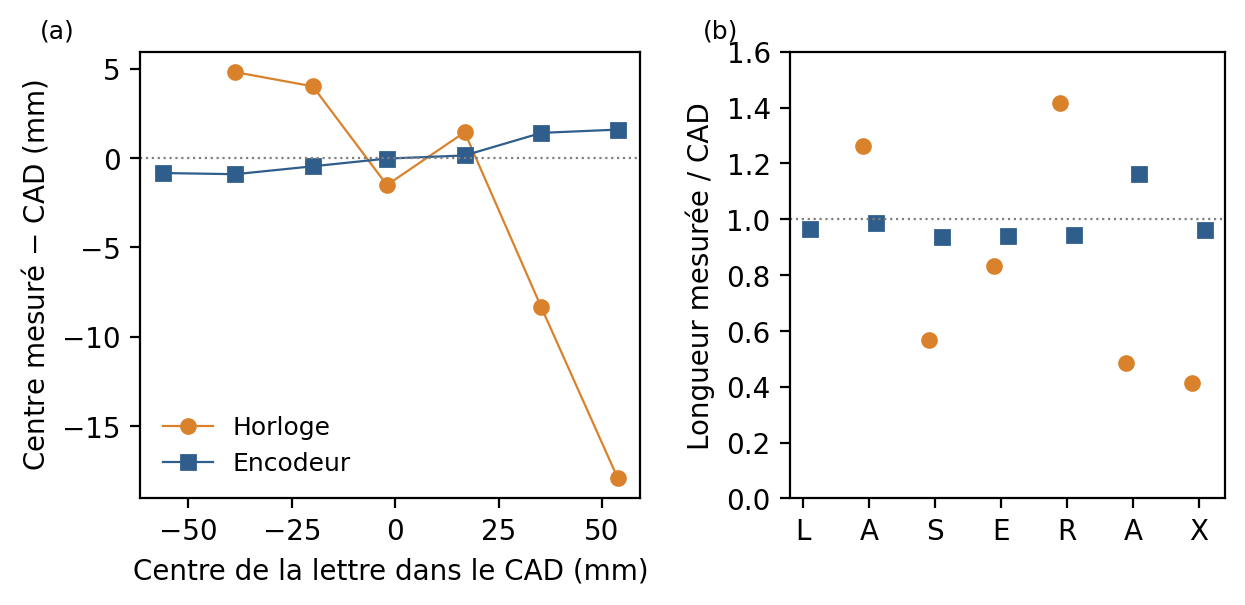
\includegraphics[width=0.82\textwidth]{../figures/03_positions_lettres.png}
    \caption{Écart entre le centre mesuré et le centre CAD de chaque lettre (a) et rapport entre la longueur mesurée et la longueur CAD (b), sans encodeur (cercles orange) et avec encodeur (carrés bleus).}
    \label{fig:positions}
\end{figure}

L'encodeur a laissé 29 positions vides sur 578 (5~\%), en 13 trous d'au plus 5 positions (1,25~mm). Ils sont presque tous dans une même zone, où la sonde a avancé en moyenne de 1,9 position entre deux tirs.

\section{Discussion}
\label{sec:discussion}

\subsubsection*{Profondeur et vitesse du son}
En profondeur, la reconstruction est bonne: les quatre grandeurs du Tableau~\ref{tab:profondeur} correspondent au CAD à l'intérieur de leur incertitude, qui est dominée par la vitesse du son. L'écart entre les deux échos de fond permet de vérifier cette vitesse, parce qu'il ne dépend pas du zéro de profondeur. Il vaut 9,68~mm dans les deux acquisitions, alors que la plaque fait 9,50~mm. Pour que cet écart donne 9,50~mm, il faudrait une vitesse de $6330 \pm 60~\text{m/s}$, proche de la valeur nominale de 6320~m/s et loin des 6451~m/s de la calibration. La calibration de vitesse aurait donc dû être faite avec le bloc utilisé lors des mesures, et non avec un bloc de calibration.

\subsubsection*{Le long de la sonde}
Le long de la sonde, les positions viennent de l'électronique: chaque faisceau est décalé de 0,6~mm, peu importe comment la main bouge. C'est pourquoi les hauteurs des lettres sont semblables dans les deux acquisitions. Pour l'acquisition avec encodeur, le rail a aussi gardé la sonde à la même position en largeur pendant tout le balayage: le décalage des lettres le long de la sonde ne varie que de 1,1~mm d'une lettre à l'autre, contre 2,7~mm sans encodeur. L'encodeur améliore donc la précision le long du balayage, et le rail la précision le long de la sonde. Les hauteurs les plus éloignées du CAD sont celles du L (+2,4~mm) et du X (+1,1~mm) avec l'encodeur. Leur bas est proche du bord du bloc, où l'écho de fond baisse déjà parce qu'une partie de l'ouverture n'est plus sur la pièce, étant donné que la sonde est plus longue que la largeur du bloc.

\subsubsection*{Le long du balayage}
Sans encodeur, la reconstruction suppose une vitesse constante de 5~mm/s. Une erreur constante sur la vitesse ne ferait que changer l'échelle, mais la main a changé de vitesse d'une lettre à l'autre, d'un facteur 4,3 entre la plus lente et la plus rapide, et parfois même à l'intérieur d'une lettre, comme pour le R. Chaque lettre a donc sa propre échelle, et aucun ajustement global ne peut corriger cette distorsion.

Avec l'encodeur, cette distorsion disparaît: l'écart RMS des centres (0,28~mm) est de l'ordre du pas de balayage. Il reste une erreur d'échelle de $2{,}4 \pm 0{,}3~\%$ qui touche toutes les distances. Elle vient très probablement de la calibration de l'encodeur: la résolution entrée était de 18,68~pas/mm, alors que les données indiquent plutôt $18{,}68 \times 1{,}024 = 19{,}13~\text{pas/mm}$. Une erreur de 2,4~mm sur une distance de calibration de 100~mm suffit pour l'expliquer. Avec la résolution par défaut de 20~pas/mm, l'erreur aurait été de $-4{,}3~\%$, donc la calibration a quand même aidé.

\subsubsection*{Trous de l'encodeur}
Dans la zone des trous, 1,9 position par tir correspond à une vitesse d'environ $1{,}9 \times 0{,}25~\text{mm} \times 51~\text{Hz} \approx 24~\text{mm/s}$. C'est le double de la vitesse maximale de l'équation~\ref{eq:vmax}, $v_{\max} = 0{,}25~\text{mm} \times 51~\text{Hz} = 12{,}8~\text{mm/s}$. Les 51~Hz viennent de la fréquence de répétition des tirs (2500~Hz) partagée entre les 49 faisceaux.

\section{Conclusion}
\label{sec:conclusion}

Le Topaz et sa sonde de 64 éléments ont permis de reconstruire en 3D un relief machiné, lu à travers 9,5~mm d'aluminium. En profondeur, les deux acquisitions donnent le dessus de la plaque et le dessus des lettres à environ 0,3~mm près. L'écart entre les deux échos de fond indique toutefois que la vitesse calibrée était environ 2~\% trop haute. Le long de la sonde, la position est fixée par l'électronique et les hauteurs des lettres sont bonnes dans les deux cas. Le long du balayage, l'encodeur fait toute la différence: sans lui, la vitesse irrégulière d'un déplacement à la main déforme les lettres de $-59$ à $+80~\%$, et avec lui il ne reste qu'une erreur d'échelle de 2,4~\%, qui vient de sa calibration. Il faut quand même déplacer la sonde à une vitesse sous 12,8~mm/s pour éviter les trous. Une prochaine expérience pourrait utiliser une calibration propre à l'échantillon utilisé lors des acquisitions. Aussi, le même montage pourrait servir à mesurer la taille d'un vrai défaut caché, par exemple un trou percé dans un bloc, et à vérifier la précision obtenue ici.

\renewcommand{\refname}{Bibliographie}
\begin{thebibliography}{9}

\bibitem{drinkwater}
Drinkwater, B.W. et Wilcox, P.D. « Ultrasonic arrays for non-destructive evaluation: A review ». \textit{NDT \& E International}, vol.~39, n\textsuperscript{o}~7, p.~525-541, 2006.

\bibitem{olympus}
Olympus NDT (R/D Tech). \textit{Introduction to Phased Array Ultrasonic Technology Applications: R/D Tech Guideline}. Waltham (MA), Olympus NDT, 2004.

\bibitem{krautkramer}
Krautkrämer, J. et Krautkrämer, H. \textit{Ultrasonic Testing of Materials}, 4\textsuperscript{e} édition. Springer-Verlag, Berlin, 1990.

\bibitem{protocole_topaz}
Brodeur, L-F. et Larouche-Tremblay, S. \textit{GPH-3000, Contrôle non destructif des matériaux: Utilisation du Topaz (ultrasons phase array)}, version A26, 2026 (Annexe~\ref{ann:protocole}).

\bibitem{zetec}
Zetec, Inc. \textit{TOPAZ User Manual}, révision 10046055-R08.

\bibitem{somer}
Somer, J.C. « Electronic sector scanning for ultrasonic diagnosis ». \textit{Ultrasonics}, vol.~6, n\textsuperscript{o}~3, p.~153-159, 1968.

\end{thebibliography}

% ------------------------------------------------------------------ annexes
\clearpage
\appendix
\makeatletter
\renewcommand{\@seccntformat}[1]{Annexe~\csname the#1\endcsname:\ }
\makeatother

\thispagestyle{empty}
\vspace*{\fill}
\begin{center}
\refstepcounter{section}
\label{ann:protocole}
\addcontentsline{toc}{section}{Annexe~\thesection: Protocole d'utilisation du Topaz}
{\Huge \textbf{Annexe~\thesection}}\\[1.2em]
{\LARGE Protocole d'utilisation du Topaz}\\[0.6em]
{\large (ultrasons phase array)}
\end{center}
\vspace*{\fill}

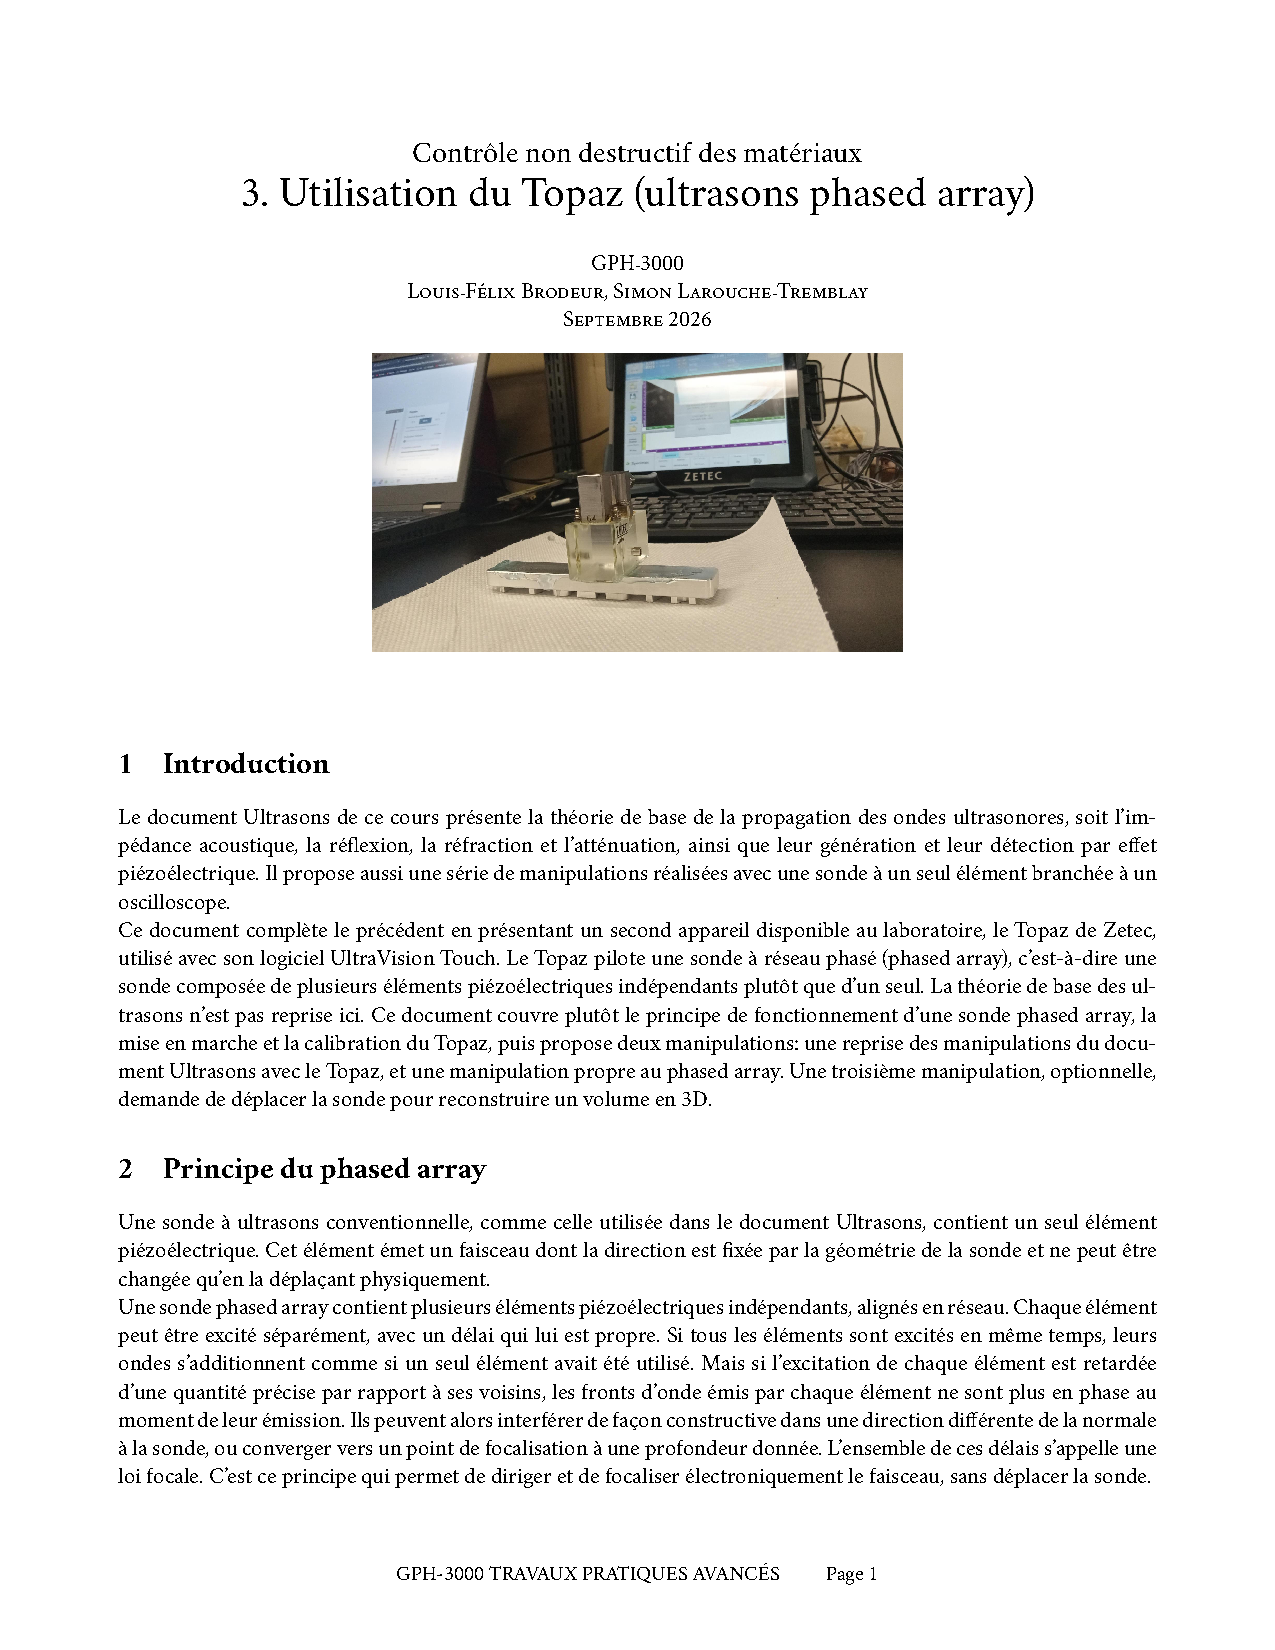
\includepdf[pages=-]{protocole_topaz/Guide_Topaz_PhasedArray_A26.pdf}

\end{document}
